\documentclass{sigchi-ext}
% Please be sure that you have the dependencies (i.e., additional
% LaTeX packages) to compile this example.
\usepackage[T1]{fontenc}
\usepackage{textcomp}
\usepackage[scaled=.92]{helvet} % for proper fonts
\usepackage{graphicx} % for EPS use the graphics package instead
\usepackage{balance}  % for useful for balancing the last columns
\usepackage{booktabs} % for pretty table rules
\usepackage{ccicons}  % for Creative Commons citation icons
\usepackage{ragged2e} % for tighter hyphenation

% Some optional stuff you might like/need.
% \usepackage{marginnote} 
% \usepackage[shortlabels]{enumitem}
% \usepackage{paralist}
% \usepackage[utf8]{inputenc} % for a UTF8 editor only

%% EXAMPLE BEGIN -- HOW TO OVERRIDE THE DEFAULT COPYRIGHT STRIP --
% \copyrightinfo{Permission to make digital or hard copies of all or
% part of this work for personal or classroom use is granted without
% fee provided that copies are not made or distributed for profit or
% commercial advantage and that copies bear this notice and the full
% citation on the first page. Copyrights for components of this work
% owned by others than ACM must be honored. Abstracting with credit is
% permitted. To copy otherwise, or republish, to post on servers or to
% redistribute to lists, requires prior specific permission and/or a
% fee. Request permissions from permissions@acm.org.\\
% {\emph{CHI'14}}, April 26--May 1, 2014, Toronto, Canada. \\
% Copyright \copyright~2014 ACM ISBN/14/04...\$15.00. \\
% DOI string from ACM form confirmation}
%% EXAMPLE END

% Paper metadata (use plain text, for PDF inclusion and later
% re-using, if desired).  Use \emtpyauthor when submitting for review
% so you remain anonymous.
\def\plaintitle{Examining Marginalization in the Financial Industry Related to Conversational Agents} \def\plainauthor{Christina Wei, Anastasia Kuzminykh}
\def\emptyauthor{}
\def\plainkeywords{conversational user interfaces; chatbot; financial industry;  marginalization}
\def\plaingeneralterms{conversational user interfaces; chatbot; financial industry;  marginalization}

\title{Examining Marginalization in the Financial Industry Related to Conversational Agents}

\numberofauthors{2}
% Notice how author names are alternately typesetted to appear ordered
% in 2-column format; i.e., the first 4 autors on the first column and
% the other 4 auhors on the second column. Actually, it's up to you to
% strictly adhere to this author notation.
\author{%
  \alignauthor{%
    \textbf{Christina Wei}\\
    \affaddr{University of Toronto} \\
    \affaddr{Toronto, Canada} \\
    \email{christina.wei@mail.utoronto.ca}
  } 
  \vfil
  \alignauthor{%
    \textbf{Anastasia Kuzminykh}\\
    \affaddr{University of Toronto}}\\
    \affaddr{Toronto, Canada} \\
    \email{anastasia.kuzminykh@utoronto.ca}
}

% Make sure hyperref comes last of your loaded packages, to give it a
% fighting chance of not being over-written, since its job is to
% redefine many LaTeX commands.
\definecolor{linkColor}{RGB}{6,125,233}
\hypersetup{%
  pdftitle={\plaintitle},
%  pdfauthor={\plainauthor},
  pdfauthor={\emptyauthor},
  pdfkeywords={\plainkeywords},
  bookmarksnumbered,
  pdfstartview={FitH},
  colorlinks,
  citecolor=black,
  filecolor=black,
  linkcolor=black,
  urlcolor=linkColor,
  breaklinks=true,
}

% \reversemarginpar%

\begin{document}

%% For the camera ready, use the commands provided by the ACM in the Permission Release Form.
\CopyrightYear{2022}
\setcopyright{rightsretained}
\conferenceinfo{CHI'23,}{April  23--28, 2023, Hamburg, Germany}
\isbn{978-1-4503-6819-3/20/04}
\doi{https://doi.org/10.1145/3334480.XXXXXXX}
%% Then override the default copyright message with the \acmcopyright command.
\copyrightinfo{\acmcopyright}


\maketitle

% Uncomment to disable hyphenation (not recommended)
% https://twitter.com/anjirokhan/status/546046683331973120
\RaggedRight{} 

% Do not change the page size or page settings.
\begin{abstract}
Current conversational agents in the financial sector are predominately focused on handling transactional inquiries in the customer service domain. This leads to marginalization of customer service employees, reinforcing the societal bias that their work is perceived as low value. There are also ethical issues in dehumanizing the work done by these workers, as well as reinforcing existing stereotypes through the use of female avatars. These conversational agents also reinforces the product differentiation based on wealth by digitizing services for general customers. We urge designers to beware of these problems and to leverage conversational agents for more inclusive design.
\end{abstract}

\keywords{\plainkeywords}

% ACM Classfication

\begin{CCSXML}
<ccs2012>
<concept>
  <concept_id>10003120.10003121</concept_id>
  <concept_desc>Human-centered computing~Human computer interaction (HCI)</concept_desc>
  <concept_significance>500</concept_significance>
</concept>
<concept>
    <concept_id>10003120.10003121.10003124.10010870</concept_id>
    <concept_desc>Human-centered computing~Natural language interfaces</concept_desc>
    <concept_significance>500</concept_significance>
</concept>
</ccs2012>
\end{CCSXML}

\ccsdesc[500]{Human-centered computing~Human computer interaction (HCI)}
\ccsdesc[500]{Human-centered computing~Natural language interfaces}

% Print the classficiation codes
\printccsdesc
%Please use the 2012 Classifiers and see this link to embed them in the text: %\url{https://dl.acm.org/ccs/ccs_flat.cfm}


\section{Introduction}

Financial decisions are among the most complex and consequential decisions we make in our lives. Many individuals need assistance to make these decisions, as the majority of Americans report feeling anxious about their financial situation \cite{capitalone2020}. The recent advancements in financial technology (FinTech) such as the introduction of robo-advisors helps to commoditize personal advice services that are were previously only accessible to high net worth individuals \cite{philippon2019fintech}. Conversational agents also has the potential to contribute to better financial inclusion, as their ability to communicate with users using natural language is well suited to support users in their decision making process \cite{volkel2021eliciting}. However, the opportunities to create chatbots for more complex decision-making tasks like financial decisions are still largely under-explored \cite{reicherts2022extending}. Instead, financial industry has mainly focused on implementing chatbots to handle transactional inquiries in the customer service context, such as Eno the Capital One Assistant\footnote{https://www.capitalone.com/digital/eno/}. While these agents are beneficial for financial institutions, they lead to discrimination problems within the industry as well as for customers.

In this paper, we first spotlight the issue of marginalizing employees through the augmentation of customer services capabilities using conversational agents. We then discuss the role of these agents in reinforcing the existing structure of wealth-based service differentiation, widening the access gap to personalized assistance between general and high net worth customers. Lastly, we highlight areas that conversational agents can be used to increase financial inclusion.


\section{Marginalization of Human Labour}

\begin{marginfigure}[-17pc]
  \begin{minipage}{\marginparwidth}
    \centering
    
\includegraphics[width=0.8\marginparwidth]{figures/chatbot.png}
    \caption{Banking and finance conversational agents from Chatbot Guide \cite{chatbotguide}}
    \label{fig:chatbots}
  \end{minipage}
\end{marginfigure}

%Because of current conversational agents are currently only equipped to perform simple transactional tasks, most companies are defaulting to build digital assistants to augment their existing customer service capabilities. This is evident in the financial industry, 
Surveying the landscape conversational agents used in banking and finance, most companies are implementing chatbots to support transactional inquiries such as checking account balance or to make a payment \cite{chatbotguide}. Financial institutions' collective choices to augment transactional customer service capabilities with virtual agents is an evidence of the reification of labour politics that is deeply rooted in our culture. There is a societal bias that customer service is perceived as low value and repetitive work, therefore it is easier to automate as compared to higher value work performed by financial advisors \cite{dhaliwal2022cyber}. Due to the lower social status of the customer service workers, they have limited ability to fight back against the augmentation of their jobs. However, if one objectively analyzes the tasks performed by financial advisors and customer service representatives, both roles have elements that can be automated by machines like conversational agents. This augmentation of customer services with conversational agents also creates a dangerous self-reinforcing cycle. Because customer service is perceived as low value work, there are more automation built to augment their capabilities. Now that there are more automatic capabilities built for customer services, it reinforces the stereotype that this type of work is low value and can be automated. With the automation of capabilities, it also introduces the issue of hiding human labour behind machines.

There are ethical concerns with the representation of customer service work through conversational agents. Grudin and Jacques \cite{grudin2019chatbots} bring up the issues in human-chatbot teams for human agents to jump in and handle inquiries that conversational agents are unable to answer. If conversational agents are not designed properly, customers may not be able to distinguish between human vs. virtual agents, therefore mistakenly attributing human work to the machine. In extreme cases, companies may be deliberately hiding human labour behind the facade of conversational agents, disguising customer service representatives' work as the agents' algorithms. Also, there is the problem of how conversational agents are portraying the customer service worker. Through our analysis of the 34 agents listed in Chatbot Guide for Banking and Finance Industry \cite{chatbotguide} (\autoref{fig:chatbots}) , most of them used abstract avatars or the company's logo to represent the virtual assistant. The lack of human resemblance in these chatbots dehumanizes the role of customer service representatives, treating them as commodities who are indistinguishable and interchangeable with each other. Out of the conversational agents listed in Chatbot Guide, five of them used typical female names (Erica from Bank of America\footnote{https://www.chatbotguide.org/bank-of-america-bot}, Sara from Commercial Bank of Dubai\footnote{https://www.chatbotguide.org/commercial-bank-of-dubai-bot}, Ada from Diamond Bank\footnote{https://www.chatbotguide.org/diamond-bank-bot}, Eva from HDFC Bank\footnote{https://www.chatbotguide.org/hdfc-bot}, and Hannah from M\&S Bank\footnote{https://www.chatbotguide.org/ms-bank-bot}) compare to only one agent using a typical male name (Lionel from ING\footnote{https://www.chatbotguide.org/ing-bot}). Some agents with female names are also associated with human-like avatars depicted with typical female features (\autoref{fig:female-avatars}). This analysis illustrates the bias of choosing female personas for conversational agents, which may be reinforcing harmful gender stereotypes such as subservient attitude to customer service representatives \cite{ruane2019conversational}.

\begin{marginfigure}[3pc]
  \begin{minipage}{\marginparwidth}
    \centering
    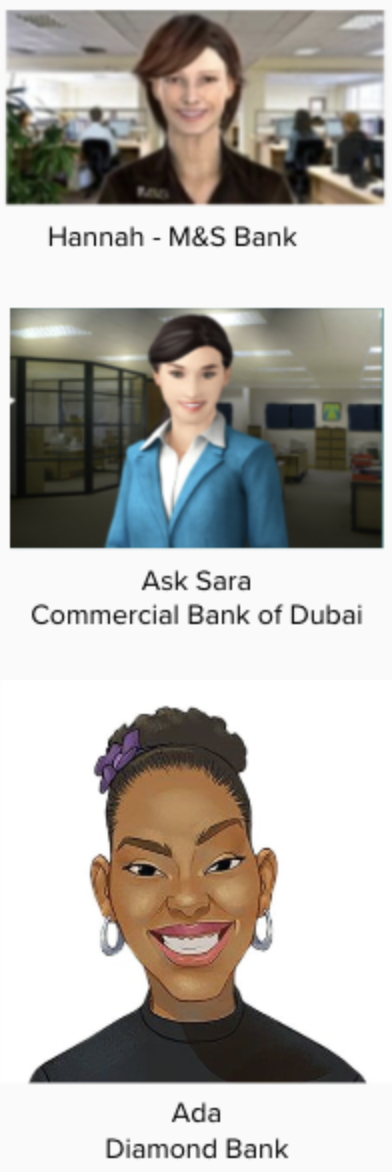
\includegraphics[width=0.8\marginparwidth]{figures/avatars.png}
    \caption{Banking and finance bots using female avatars}
    \label{fig:female-avatars}
  \end{minipage}
\end{marginfigure}


\section{Reinforcing Wealth-Based Service Differentiation}

Using conversational agents to augment customer service capabilities reinforces the divide between services available to general customers vs. high net worth individuals. Virtual agents are usually built for services available to general customers, yield positive returns on investment on commonly asked inquiries. On the other hand, dedicated services provided to high net worth individuals usually do not invest in conversational agents, as their value proposition is the white glove support model to build personal relationships with customers. The notion that these specialized and dedicated services can be augmented by virtual assistants diminishes their perceived value. As such, there is a divide between the digitization of the services available to customers, and the personalized services that high net worth individuals continue to enjoy. For general customers, it is common to be interfacing with automated algorithms as the first interaction point. For example, when calling into contact centres, customers need to first navigate through an Interactive Voice Response (IVR) system before they can reach a human customer service representative. Similarly, conversational agents are being advertised and used as a first point of contact to help customers on digital channels \cite{revechat}. A customer will only be transferred to a human representative if the virtual agent's algorithm determines that it cannot handle the client's inquiry. This reduces the access to personalized help for general customers, potentially limiting flexibility on their financial products. These limitations do not apply for high net worth individuals as they have access to dedicated teams to assist them with their financial needs. Thus, digital tools like conversational agents are reinforcing and potentially even deepening the divide in services between general vs. high net-worth customers.


\section{Moving Towards Inclusive Design}

While the current implementations of conversational agents have marginalizing effects in the financial industry, they can also be used for more inclusive design. One example is to use virtual agents to reduce the access segregation of financial products. In financial services, many products are transacted through intermediaries, such as financial advisors purchasing mutual funds on behalf of their customers. Customers' access to financial products depend on intermediaries' regulatory licenses and product coverage. For example, a broker may be licensed to offer insurance products and not mutual funds, but their customers may not be aware of this limitation and potentially missing out on access to broader range of products. Conversational agents can be used to educate customers on the full spectrum of financial products that are available in the market, as well as connecting them with appropriate financial intermediaries to address their financial needs. Also, as conversational agents evolve to handle more complicated conversations, we can implement more personalized advice solutions typically available to high net worth individuals for general customers, reducing the gap of wealth-based service differentiation. This work is already happening in FinTech through robo-advisor capabilities \cite{philippon2019fintech}, we can further assist users with their financial decision making by augmenting these services using conversational agents. 


\section{Closing Remarks}

This paper discusses various aspects of marginalization by conversational agents in the financial industry. Specifically, there are marginalizing effects for both users of conversational agents and the workers whose jobs are affected by these agents. We can leverage Sin et al.\cite{sin2021digital}'s digital design marginalization framework to avoid digitally marginalizing groups of users and design inclusive digital interfaces. Specifically for the financial industry, we urge the conversational user interface community to investigate agents supporting users in their financial decision-making process in order to narrow the wealth-based access gap for personalized financial advice.

\balance{} 

\bibliographystyle{SIGCHI-Reference-Format}
\bibliography{reference}

\end{document}

%%% Local Variables:
%%% mode: latex
%%% TeX-master: t
%%% End:
